\documentclass[10pt,conference,compsocconf]{IEEEtran}
\usepackage{hyperref}
\usepackage{graphicx}   % For figure environment
\usepackage{subfigure}
\usepackage{titling} % Customizing the title section
\usepackage{dblfloatfix}    % To enable figures at the bottom of page
\usepackage{kantlipsum}     % for random text
\usepackage{todonotes}
\usepackage{multirow}
\usepackage[margin=0.9in]{geometry}
\usepackage[english]{babel}
\usepackage{caption,setspace}

\usepackage{dsfont}

\usepackage{array}
\newcolumntype{P}[1]{>{\centering\arraybackslash}p{#1}}
\newcolumntype{M}[1]{>{\centering\arraybackslash}m{#1}}
\begin{document}
        
\pretitle{\begin{center}\Huge\bfseries} % Article title formatting
\posttitle{\end{center}} % Article title closing formatting
\title{Hotgrad: a deep learning framework}
\author{
        % Your name
        \textsc{Niccol\`{o} Sacchi, Succa Riccardo \& Marco Zoveralli}
        \normalsize{} \\
        % Your institution
        \normalsize \'{E}cole polytechnique f\'{e}d\'{e}rale de Lausanne
}
\maketitle
\begin{abstract}
  This project aims to contruct a deep learning framework based only on pytorch Tensors and standard math libraries. Our framework has been designed to simplify the basic operations of a neural network, in particular forward and backward functions, that have a foundamental role in the way a network operates.
  This framework is then used to generate a simple deep neural network and test it with an internal dataset. We compare the results with some baselines from the sklearn library.
  Future development can be easily realized thanks to the modularity of the code.
\end{abstract}
\section{Introduction}
    
   In the development of a deep learning framework, it is crucial to provide the final user an highly versatile and efficient set of modules, that can be freely combined in order to construct complex neural networks. Our approach focused on this features and aimed to simplify the network basic operations. In particular, the functioning of a neural network is based on two main steps, the forward and the backward passes, that allow the network to compute the output (given an input) and to train its parameters in order to increase the accurancy.\\
   Each layer of the fully connected network consists in a series of nodes, each of them connected to the entire set of nodes of the previous layer with a series of weights. During the forward pass, an input is given to the first layer and it is propagated to all the subsequent layers by multiplying it with the weights and additionally summing biases. In order to introduce a non-linearity into the network, each layer usually applies a non-linear function after this operation. This non-linear function avoids that the output can be reproduced from a linear combination of the inputs, which leads to poor accuracy when the input dataset is not linearly separable. From a mathematical point of view, the forward pass can be seen as a series of function applied to the input:\\
   \[y = f(g(h(...(x)))\]\\
   All the weights and biases of the network are initially set to a uniform value from the interval $(-1/\sqrt{d}, 1/\sqrt{d}) $ (where d is the layer's input dimension), so at the beginning the accurancy of the network is around 50\%. In order to adjust all the layers' parameters, modern neural networks use the \textit{back propagation}, based on the chain rule. The back propagation aims to compute the gradient of the loss function with respect to the input and use it to distribute the error to all the layers. In particular, the loss function fist calculates how much the output of the network differs from the expected output. Then, the gradient of the loss is propagated back through the network and associates a value to each neuron, which reflects how much the neuron contributes to the total error. Finally, an optimization algorithm uses this error to update the weights and biases of each layer, in order to minimize the loss function:\\
    \[w = w + \eta\nabla L(w)\]
    \[b = b + \eta\nabla L(b)\]\\
   where \textit{w} and \textit{b} indicates the weight and biases for each layer.

The following section describes the implementation design choices behined our framework. Then, the structure of the code is described in section 3. Section 4 contains a description of the testing methodology, i.e., the dataset used to run the network, the network that was built through our framework, and the comparisons with other common models. Section 5 concludes this report by mentioning the achieved goals and the possible future developments.
\section{Implementation}
	Since this project provided the structure of the final neural network, the simplest approach to the problem would have been to contruct one class containing all the parameters of the layers and manually write the forward and backward pass. This would lead to a simple but difficult-to-read implemetation, without any possibility to expand or modify the network. We immediately discard this option and we instead focused on a modular solution.
	Having in mind how a network operates, we can notice that in order to calculate the backward pass, each operation needs to keep track of the inputs that were passed to it, so that it can easily compute the derivative of the loss wrt them. Consequently, we started the implementation of the base operations, in particular addition, subtraction, multiplication, matrix multiplication, pow and mean, plus the activation functions ReLU and Tanh. Each of this operation saves the inputs that were passed to it and implements the forward and backward pass. On the other hand, we built the Variable class to wrap all the necessary information of a variable: the data value itself (that consists in a torch FloatTensor), the gradient and the link to the operation that generated it. This can be seen as a bottom up approach, where we decompose to problem starting from the very basic operations, and then construct more complex modules on top of them. The graph shown in picture 1 explains how this modules and variables are used to compute the forward and backward pass.

	\begin{center}
		\captionsetup{type=figure}
		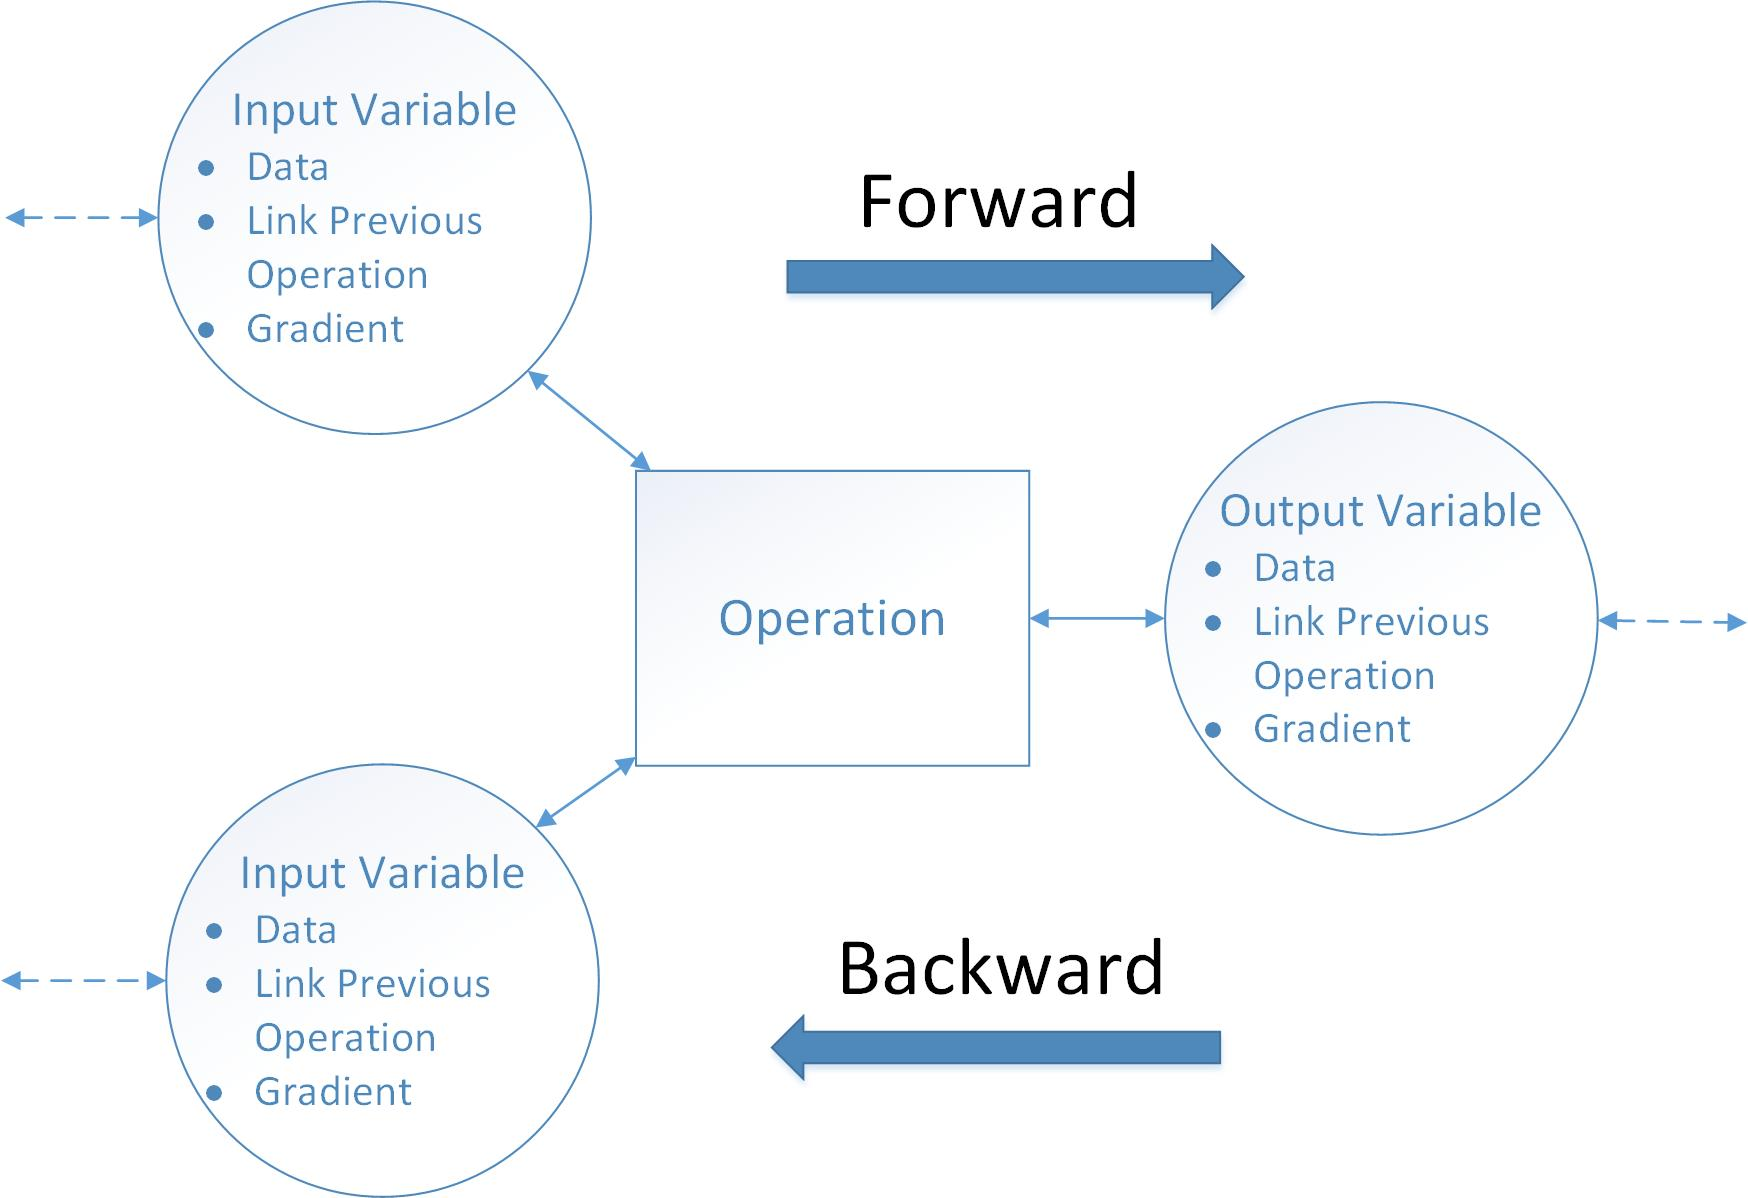
\includegraphics[width=0.5\textwidth]{img/ForwardBackward.jpg}
		\label{fig:ForwardBackward}
		\caption {Forward: The Operation Module generates a new Variable, containing the result and the link to it. Backward: The Operation Module computes the new gradient and sends it to the Input Variables.}
	\end{center}

	In the forward pass, the operation takes its inputs as Variables and produces a new Variable with the data field set to the result of the operation itself; the new Variable also contains the link to the function that generated it. Then, this new Variable can be used as input for any subsequent operation, and the process is repeated.  Starting from the input, this chain of operations continues until the final layer of the network. 
	In the backward pass, instead, each operation receives a gradient as parameter from the output Variable, calculates the derivative of the gradient wrt the inputs and then back propagates the new gradient to the input Variables. Inside the Variable itself, the gradient is accumulated in the \textit{grad} field and then passed to the previous operation if necessary. In the global point of view of the network, we first calculate the initial gradient with the loss function applied to the output and then we back propagate the gradient to each layer until we reach the input.
        
        
\section{Code Structure}
We now describe in details the structure of the code and classes.

\begin{itemize}
	\item Module: this file contains the abstract class Module, with the basic funcions that each module will implement, in particular the forward and backward pass. This Module class is extended by two other classes, Module2Operands and Module1Operand, that distinguish between operation that requirest one or two inputs. 
	
	\item Exception: contains the exceptions needed to handle the errors.
	
	\item Optimizers: as optimizer, we implemented the Stocastic Gradient Descend (SDG), initialized with a learning rate parameter. The function \textit{set\_params} allows us to pass the list of all the parameters of the network that will require an update, after the gradient is computed in the backward pass. The update itself of the parameters is performed by the \textit{step} function.
	
	\item Sequential: this module is used as a container of other modules. It receives as input the list of modules that compose the network, the loss criterion and the optimizer. Unlike the other modules, Sequential doesn't implement the backward pass, but instead it has a \textit{fit} function that is used to train the network, given an input train and input target. More specifically, the fit function iterates through a number of epochs and compute the loss wrt the input; then the optimizer is used to update (step function) the parameters of the modules. We also added the \textit{batch\_size} parameter to the fit function, in order to speed up the performance by computing the loss with just a portion of the input: in this way, the parameters are optimized every batch size (approximizing the gradient) and not with the entire train set.
	
	\item Variable: this class is the wrapper class for the torch FloatTensor. It is used to contain the data value itself and other parameters in order to exploit the backpropagation:
	\begin{itemize}
		\item \textit{requires\_grad} is used to know if we have to calcualte the gradient for this variable and propagate it back
		\item \textit{grad} contains the gradient
		\item \textit{previous\_op} is the link to the function that generated this Variable
	\end{itemize}
	With this additional information, the backward pass is just a recursive call to the backward function of the previous operation, passing the grad as parameter. 
	
	\item Functions: the folders contain different modules that implements the basic functions. Table \ref{tab:modules} describes the content in details.
\end{itemize}
We also added the broadcasting functionality to the basic operations, which is the possibility to expand their arguments and make them of the same size. This functionality was required inside the Linear module, where we add a bias to the multiplication between input and weight matrix.
In the forward pass, this operation is trivially handled by the broadcast property of pytorch Tensors. In the backward pass, instead, if the gradient received by a Variable has not the same size of the data field, we must reshape it before the addition with the Variable's grad. This operation is easily implemented by summing the gradient over the dimensions that do not match. The property derives from the mathematical formula
\[\frac{d}{dx}f(x,y)|_{x=y} = \frac{d}{dx}f(x,y) + \frac{d}{dy}f(x,y)\]
When a variable is broadcasted, the dimensions that are expanded contains replicated values. Consequently, the derivative of the gradient can be seen as the sum of the derivatives along the axes that were replicated.\\
\begin{table*}
\caption{Modules}
\label{tab:modules}
\begin{tabular}{ | c | c | p{10cm} | c | } 
\hline
Module & Classes & Description & Forward  \\
\hline
\multirow{2}{4em}{Activations} 
& ReLU & Implements the rectified linear unit, extending the Module1Operands & $f(x) = max(0, x)$  \\
& Tanh & Hyperbolic tangent function that extend the Module1Operands & $f(x) = tanh(x)$ \\
\hline
\multirow{6}{4em}{Operands}
& Add & \multirow{6}{30em}{All these classes extend Module2Operands or Module1Operands depending on the number of inputs. They implement the forward and backward pass. } & $f(x, y) = x + y$ \\
& Sub & & $f(x, y) = x - y$ \\ 
& Mul & & $f(x, y) = x \odot y$ \\ 
& MatMul & & $f(x, y) = x * y$ \\ 
& Pow & & $f(x, exp) = x^{exp}$ \\ 
& Mean & & $\frac{1}{N} \sum_{i=1}^N x_i$ \\
\hline
Layers & Linear & The Linear module is a wrapper of two operation: multiplication of the weights and sum of the biases. & $f(x) = w*x + b$ \\ 
\hline
Losses & MSE & The mean square error extend the Module2Operands & $\frac{1}{N} \sum_{i=1}^N (x_i - \overline{x})^2$  \\ 
\hline
\end{tabular}
\end{table*}

\section{Test}
%next steps and conclusions 
% indexing, convolutional
 

In this section we provide the description of the used dataset and the network built with our framework. Then, the validity of the built model is shown by comparing it with well-known baselines.

\subsection{Dataset}
The dataset consists of a training set and a test set of 1000 points each. These points are sampled uniformly in [0, 1], and they are labeled with 0 if they end up out of the disk of radius \( \frac{1}{\sqrt{2\pi}} \) (label is 1 otherwise). The following exhibit - which represents the train set used during the testing phase - contains a set of points that satisfy these properties:

\begin{center}
	\captionsetup{type=figure}
	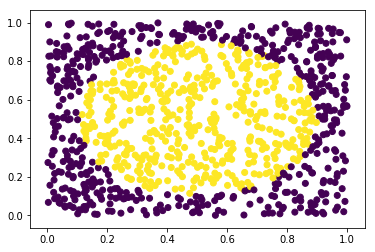
\includegraphics[width=0.5\textwidth]{img/dataset.png}
	\label{fig:dataset}
\end{center} 

For the sake of reproducibility, we used a manual seed to ensure that all the runs of the test would be the same.

\subsection{Network}
The network consists of two input units, two output units and three hidden layers of 25 units.

\begin{center}
	\captionsetup{type=figure}
	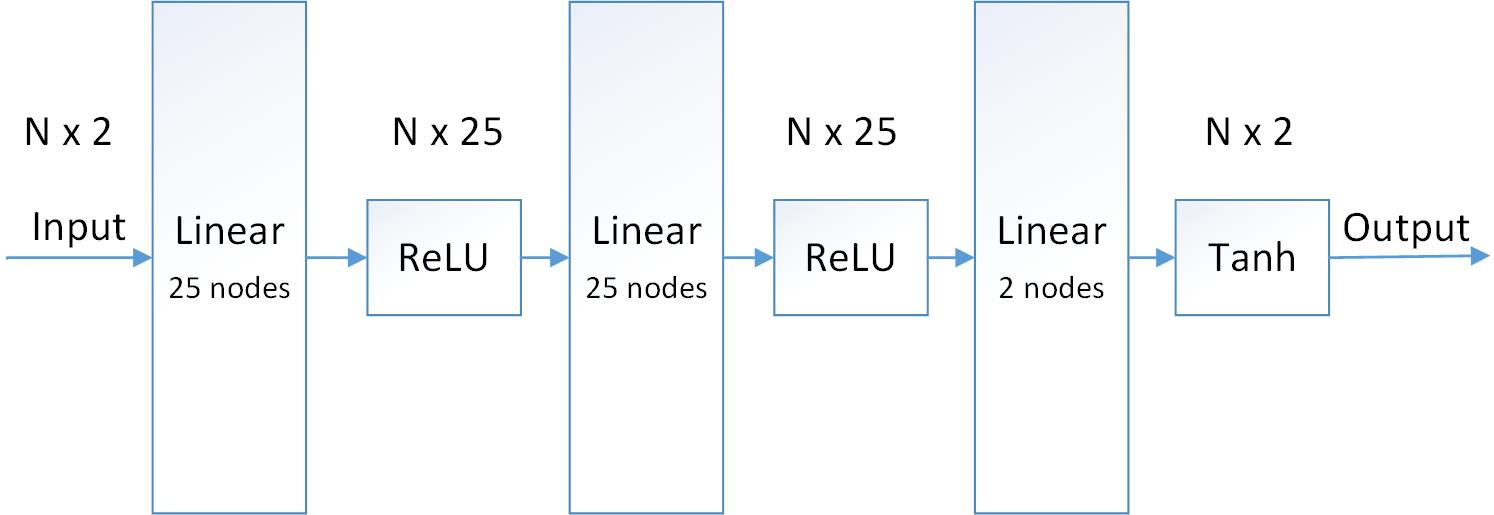
\includegraphics[width=0.5\textwidth]{img/Network.jpg}
	\label{fig:network}
\end{center} 

A Tanh activation function is used as the last component of our network. The reason behind this choice is that since we are using MSE in a classification problem, having an unbounded output would highly penalize the outcome. In fact, while the output can assume any value, the labels can only have two values. This leads to the following problem: any value that is either too high or too small is seen, by the MSE function, as something very different from the labels. 
By using the Tanh this problem is mitigated and any output value is approximated to the closest label, if its absolute value is too high.

\subsection{Model Comparison}
The accuracy of our model was tested with the aforementioned dataset. The results are quite satisfying, since the test accuracy is around 98\%.
%The following image compares our model with common baselines.
A comparison between some common baselines, the model built by using our framework and the same model built by using pytorch primitives is shown below:
\begin{center}
	\captionsetup{type=figure}
	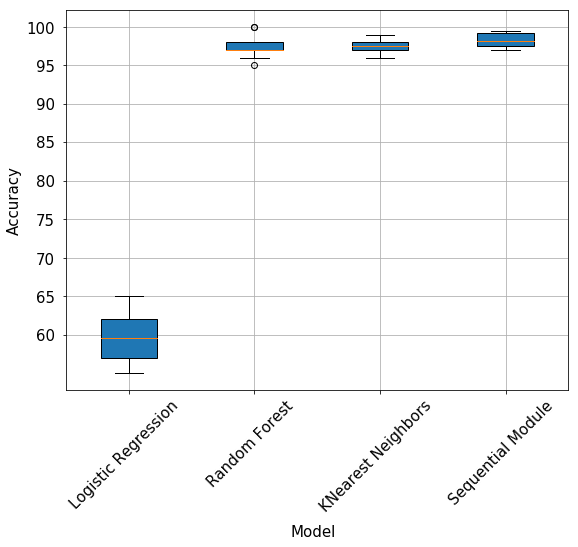
\includegraphics[width=0.5\textwidth]{img/boxplots_final.png}
	\label{fig:boxplot}
\end{center} 
Intuitively, as expected, linear classifers (K-NN, random forest) perform
reasonably well, while linear ones (logistic regression) give the worst result
because the points in the dataset are not linearly separable. In this latter case,
better performance could have been achieved through feature extraction.
It can also be seen that our model performs slightly better than any of the tested
baselines.\\
Finally, it is easy to notice that the the sequential module built by using our framework is qualitatively the same as the one built by using the pytorch primitives.
\section{Conclusion and Future Developments}
Our library is perfectly able to combine fully connected layers, to run the forward and backward passes, and to optimize the parameters through SGD and MSE.
\\Furthermore, the bottom-up approach that we followed allows us to easily develop and integrate new features. In fact, although the goal of this project was to to be able to build fully connected neural network, the framework can be easily expanded to support several other useful functionalities, such as convolutional layers, additional loss functions and optimizers, regularization (through the loss functions or optimizers), activation functions etc. This is beyond the goal of this project, but it is very useful if when dealing with more complex datasets.

\end{document}